\documentclass{beamer}
\usepackage{listings}
\lstset{
%language=C,
frame=single, 
breaklines=true,
columns=fullflexible
}
\def\inputGnumericTable{}
\usepackage{booktabs} 
\usepackage{subcaption}
\usepackage{url}
\usepackage{comment}
\usepackage{tikz}
\usepackage{tkz-euclide} % loads  TikZ and tkz-base
%\usetkzobj{all}
\usetikzlibrary{calc,math}
\usepackage{float}
\newcommand\norm[1]{\left\lVert#1\right\rVert}
\renewcommand{\vec}[1]{\mathbf{#1}}
\usepackage{color}
\usepackage{xcolor}
\usepackage[export]{adjustbox}
\usepackage[utf8]{inputenc}
\usepackage{amsmath}
\usepackage{listings}
    \usepackage{color}                                            %%
    \usepackage{array}                                            %%
    \usepackage{longtable}                                        %%
    \usepackage{calc}                                             %%
    \usepackage{multirow}                                         %%
    \usepackage{hhline}                                           %%
    \usepackage{ifthen}                                           %%
  %optionally (for landscape tables embedded in another document): %%
    \usepackage{lscape}     

\usetheme{PaloAlto}
%\usecolortheme{wolverine}

\title{Similarity of Triangles}
\author{Srihari S}
\institute{College of Engineering - Guindy}
\date{\today}
\begin{document}


\begin{frame}
\titlepage
\end{frame}
\section{Question}
\begin{frame}
\frametitle{Question}
\begin{block}{Exercise 8.1(Q no.51)}
O is a point in the interior of $\triangle ABC$. D is a point on OA. If DE $\parallel$ OB and DF $\parallel$ OC. Show that EF $\parallel$ BC.
\end{block}
\end{frame}

\section{\textbf{Construction}}
\subsection*{Codesandfigures}
\begin{frame}[fragile]
\frametitle{Codes and Figures}
\tiny
\begin{flushleft}
The python code for the figure is
\begin{lstlisting}
./codes/similartriangle.py
\end{lstlisting}
The latex- tikz code is
\begin{lstlisting}
./figs/constructionpic.tex
\end{lstlisting}
The above latex code can be compiled as standalone document
\begin{lstlisting} 
./figs/constructionpic_standalone.tex
\end{lstlisting}
\end{flushleft}.
\begin{comment}
\begin{figure}[!ht]
\begin{subfigure}{0.25\textwidth}
\includegraphics[scale=0.4]{anattemptfig.eps}
\caption{\tiny By Python}
\end{subfigure}
\end{figure}
\end{comment}
\end{frame}

\begin{frame}
\begin{figure}[!ht]
\begin{flushleft}
\begin{subfigure}{0.25\textwidth}
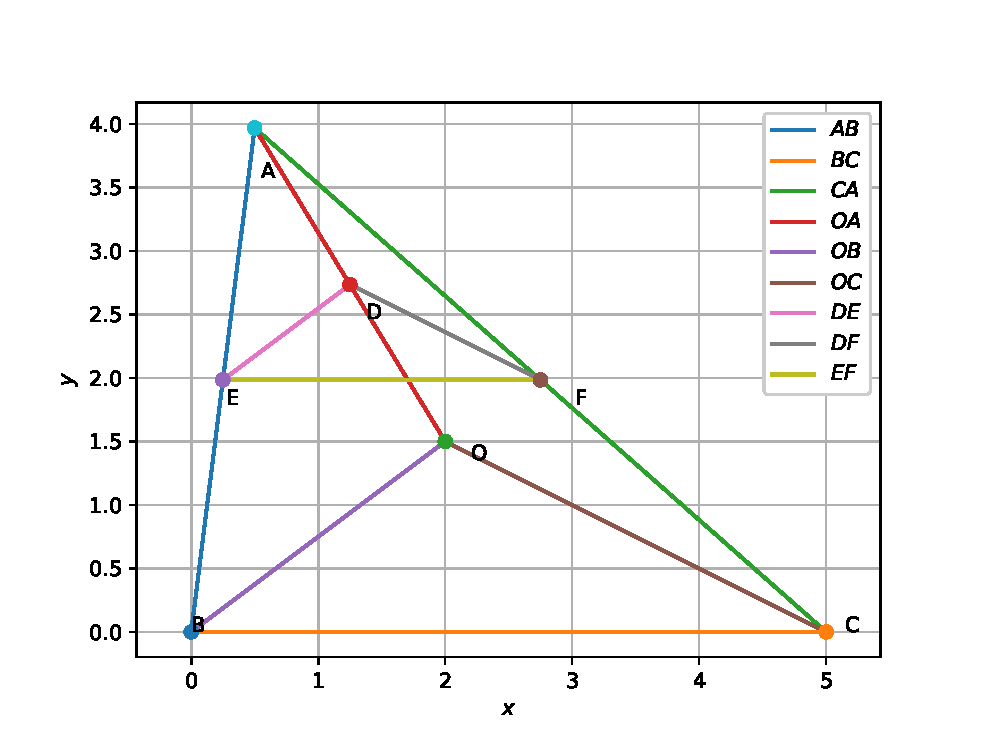
\includegraphics[scale=0.5]{./figs/similartrianglefig.eps}
\caption{\tiny By Python}
\label{fig:triabcpy}
\end{subfigure}
\end{flushleft}
\end{figure}
\end{frame}


\begin{frame}[shrink=30]

\begin{flushleft}
\begin{figure}[!ht]

%\begin{subfigure}{0.4\textwidth}
\begin{tikzpicture}
[scale=2,>=stealth,point/.style={draw,circle,fill = black,inner sep=0.5pt},]

%Triangle sides
\def\a{5}
\def\b{6}
\def\c{4}
 
%Coordinates of A
\def\p{0.5}
\def\q{{sqrt(\c^2-\p^2)}}

%Labeling points
\node (A) at (\p,\q)[point,label=above right:$A$] {};
\node (B) at (0, 0)[point,label=below left:$B$] {};
\node (C) at (\a, 0)[point,label=below right:$C$] {};
\node (O) at (2,1.5)[point,label=below:$O$]{};
%Foot of median

\node (D) at ($(A)!0.5!(O)$)[point,label=below:$D$] {};
\node (E) at ($(A)!0.5!(B)$)[point,label=left:$E$] {};
\node (F) at ($(C)!0.5!(A)$)[point,label=right:$F$] {};

%Drawing triangle ABC
\draw (A) -- node[left, xshift=-5mm,yshift=5mm] {$\textrm{c}$} (B) -- node[below, yshift=-5mm] {$\textrm{a}$} (C) -- node[above right,xshift=2mm,yshift=5mm] {$\textrm{b}$} (A);
\draw (A) -- (D) -- (O);
%Drawing medians BE and CF
\draw (D) -- (E);
\draw (D) -- (F);
\draw (O) -- (B);
\draw (O) -- (C);
%Drawing EF
\draw (E) -- (F);

%Labeling sides
%\node [right] at ($(A)!0.5!(E)$) {$\frac{b}{2}$};
%\node [right] at ($(C)!0.5!(E)$) {$\frac{b}{2}$};
%\node [left] at ($(B)!0.5!(F)$) {$\frac{c}{2}$};
%\node [left] at ($(A)!0.5!(F)$) {$\frac{c}{2}$};




%Angles
\tkzMarkAngle[size=.3](D,E,A)
\tkzMarkAngle[size=.3](O,B,A)
%
\tkzMarkAngle[size=.7](A,F,D)
\tkzMarkAngle[size=.7](A,C,O)
%%
\tkzMarkAngle[size=.2](A,D,E)
\tkzMarkAngle[size=.2](A,O,B)
%%
\tkzMarkAngle[size=.2](F,D,A)
\tkzMarkAngle[size=.2](C,O,A)
%
%\tkzMarkAngle[size=.3](E,A,D)
%\tkzMarkAngle[size=.3](D,A,F)

\begin{comment}
%Angles
\tkzMarkAngle[fill=green!60,size=.3](D,E,A)
\tkzMarkAngle[fill=green!60,size=.3](O,B,A)
%
\tkzMarkAngle[fill=red!60,size=.5](A,F,D)
\tkzMarkAngle[fill=red!60,size=.5](A,C,O)
%%
\tkzMarkAngle[fill=yellow!60,size=.2](A,D,E)
\tkzMarkAngle[fill=yellow!60,size=.2](A,O,B)
%%
\tkzMarkAngle[fill=orange!60,size=.2](F,D,A)
\tkzMarkAngle[fill=orange!60,size=.2](C,O,A)
%
\tkzMarkAngle[fill=blue!60,size=.3](E,A,D)
\tkzMarkAngle[fill=blue!60,size=.3](D,A,F)
\end{comment}
\end{tikzpicture}

\caption{ By Latex-tikz}
\label{fig:similar}
%\end{subfigure}
\end{figure}
\end{flushleft}
\end{frame}




\section*{Construction methods}
\begin{frame}[fragile]
\footnotesize
\frametitle{Construction method}
\begin{columns}
\begin{column}{0.5\textwidth}
The values used for constructing the triangles in both Python and \LaTeX{}-Tikz is given below:
\begin{table}[ht]
    \begin{center}
    	%%%%%%%%%%%%%%%%%%%%%%%%%%%%%%%%%%%%%%%%%%%%%%%%%%%%%%%%%%%%%%%%%%%%%%
%%                                                                  %%
%%  This is the header of a LaTeX2e file exported from Gnumeric.    %%
%%                                                                  %%
%%  This file can be compiled as it stands or included in another   %%
%%  LaTeX document. The table is based on the longtable package so  %%
%%  the longtable options (headers, footers...) can be set in the   %%
%%  preamble section below (see PRAMBLE).                           %%
%%                                                                  %%
%%  To include the file in another, the following two lines must be %%
%%  in the including file:                                          %%
%%        \def\inputGnumericTable{}                                 %%
%%  at the beginning of the file and:                               %%
%%        \input{name-of-this-file.tex}                             %%
%%  where the table is to be placed. Note also that the including   %%
%%  file must use the following packages for the table to be        %%
%%  rendered correctly:                                             %%
%%    \usepackage[latin1]{inputenc}                                 %%
%%    \usepackage{color}                                            %%
%%    \usepackage{array}                                            %%
%%    \usepackage{longtable}                                        %%
%%    \usepackage{calc}                                             %%
%%    \usepackage{multirow}                                         %%
%%    \usepackage{hhline}                                           %%
%%    \usepackage{ifthen}                                           %%
%%  optionally (for landscape tables embedded in another document): %%
%%    \usepackage{lscape}                                           %%
%%                                                                  %%
%%%%%%%%%%%%%%%%%%%%%%%%%%%%%%%%%%%%%%%%%%%%%%%%%%%%%%%%%%%%%%%%%%%%%%



%%  This section checks if we are begin input into another file or  %%
%%  the file will be compiled alone. First use a macro taken from   %%
%%  the TeXbook ex 7.7 (suggestion of Han-Wen Nienhuys).            %%
\def\ifundefined#1{\expandafter\ifx\csname#1\endcsname\relax}


%%  Check for the \def token for inputed files. If it is not        %%
%%  defined, the file will be processed as a standalone and the     %%
%%  preamble will be used.                                          %%
\ifundefined{inputGnumericTable}

%%  We must be able to close or not the document at the end.        %%
	\def\gnumericTableEnd{\end{document}}


%%%%%%%%%%%%%%%%%%%%%%%%%%%%%%%%%%%%%%%%%%%%%%%%%%%%%%%%%%%%%%%%%%%%%%
%%                                                                  %%
%%  This is the PREAMBLE. Change these values to get the right      %%
%%  paper size and other niceties.                                  %%
%%                                                                  %%
%%%%%%%%%%%%%%%%%%%%%%%%%%%%%%%%%%%%%%%%%%%%%%%%%%%%%%%%%%%%%%%%%%%%%%

	\documentclass[12pt%
			  %,landscape%
                    ]{report}
       \usepackage[latin1]{inputenc}
       \usepackage{fullpage}
       \usepackage{color}
       \usepackage{array}
       \usepackage{longtable}
       \usepackage{calc}
       \usepackage{multirow}
       \usepackage{hhline}
       \usepackage{ifthen}

	\begin{document}


%%  End of the preamble for the standalone. The next section is for %%
%%  documents which are included into other LaTeX2e files.          %%
\else

%%  We are not a stand alone document. For a regular table, we will %%
%%  have no preamble and only define the closing to mean nothing.   %%
    \def\gnumericTableEnd{}

%%  If we want landscape mode in an embedded document, comment out  %%
%%  the line above and uncomment the two below. The table will      %%
%%  begin on a new page and run in landscape mode.                  %%
%       \def\gnumericTableEnd{\end{landscape}}
%       \begin{landscape}


%%  End of the else clause for this file being \input.              %%
\fi

%%%%%%%%%%%%%%%%%%%%%%%%%%%%%%%%%%%%%%%%%%%%%%%%%%%%%%%%%%%%%%%%%%%%%%
%%                                                                  %%
%%  The rest is the gnumeric table, except for the closing          %%
%%  statement. Changes below will alter the table's appearance.     %%
%%                                                                  %%
%%%%%%%%%%%%%%%%%%%%%%%%%%%%%%%%%%%%%%%%%%%%%%%%%%%%%%%%%%%%%%%%%%%%%%

\providecommand{\gnumericmathit}[1]{#1} 
%%  Uncomment the next line if you would like your numbers to be in %%
%%  italics if they are italizised in the gnumeric table.           %%
%\renewcommand{\gnumericmathit}[1]{\mathit{#1}}
\providecommand{\gnumericPB}[1]%
{\let\gnumericTemp=\\#1\let\\=\gnumericTemp\hspace{0pt}}
 \ifundefined{gnumericTableWidthDefined}
        \newlength{\gnumericTableWidth}
        \newlength{\gnumericTableWidthComplete}
        \newlength{\gnumericMultiRowLength}
        \global\def\gnumericTableWidthDefined{}
 \fi
%% The following setting protects this code from babel shorthands.  %%
 \ifthenelse{\isundefined{\languageshorthands}}{}{\languageshorthands{english}}
%%  The default table format retains the relative column widths of  %%
%%  gnumeric. They can easily be changed to c, r or l. In that case %%
%%  you may want to comment out the next line and uncomment the one %%
%%  thereafter                                                      %%
\providecommand\gnumbox{\makebox[0pt]}
%%\providecommand\gnumbox[1][]{\makebox}

%% to adjust positions in multirow situations                       %%
\setlength{\bigstrutjot}{\jot}
\setlength{\extrarowheight}{\doublerulesep}

%%  The \setlongtables command keeps column widths the same across  %%
%%  pages. Simply comment out next line for varying column widths.  %%
\setlongtables

\setlength\gnumericTableWidth{%
	53pt+%
	53pt+%
0pt}
\def\gumericNumCols{2}
\setlength\gnumericTableWidthComplete{\gnumericTableWidth+%
         \tabcolsep*\gumericNumCols*2+\arrayrulewidth*\gumericNumCols}
\ifthenelse{\lengthtest{\gnumericTableWidthComplete > \linewidth}}%
         {\def\gnumericScale{\ratio{\linewidth-%
                        \tabcolsep*\gumericNumCols*2-%
                        \arrayrulewidth*\gumericNumCols}%
{\gnumericTableWidth}}}%
{\def\gnumericScale{1}}

%%%%%%%%%%%%%%%%%%%%%%%%%%%%%%%%%%%%%%%%%%%%%%%%%%%%%%%%%%%%%%%%%%%%%%
%%                                                                  %%
%% The following are the widths of the various columns. We are      %%
%% defining them here because then they are easier to change.       %%
%% Depending on the cell formats we may use them more than once.    %%
%%                                                                  %%
%%%%%%%%%%%%%%%%%%%%%%%%%%%%%%%%%%%%%%%%%%%%%%%%%%%%%%%%%%%%%%%%%%%%%%

\ifthenelse{\isundefined{\gnumericColA}}{\newlength{\gnumericColA}}{}\settowidth{\gnumericColA}{\begin{tabular}{@{}p{53pt*\gnumericScale}@{}}x\end{tabular}}
\ifthenelse{\isundefined{\gnumericColB}}{\newlength{\gnumericColB}}{}\settowidth{\gnumericColB}{\begin{tabular}{@{}p{53pt*\gnumericScale}@{}}x\end{tabular}}

\begin{tabular}[c]{%
	b{\gnumericColA}%
	b{\gnumericColB}%
	}

%%%%%%%%%%%%%%%%%%%%%%%%%%%%%%%%%%%%%%%%%%%%%%%%%%%%%%%%%%%%%%%%%%%%%%
%%  The longtable options. (Caption, headers... see Goosens, p.124) %%
%	\caption{The Table Caption.}             \\	%
% \hline	% Across the top of the table.
%%  The rest of these options are table rows which are placed on    %%
%%  the first, last or every page. Use \multicolumn if you want.    %%

%%  Header for the first page.                                      %%
%	\multicolumn{2}{c}{The First Header} \\ \hline 
%	\multicolumn{1}{c}{colTag}	%Column 1
%	&\multicolumn{1}{c}{colTag}	\\ \hline %Last column
%	\endfirsthead

%%  The running header definition.                                  %%
%	\hline
%	\multicolumn{2}{l}{\ldots\small\slshape continued} \\ \hline
%	\multicolumn{1}{c}{colTag}	%Column 1
%	&\multicolumn{1}{c}{colTag}	\\ \hline %Last column
%	\endhead

%%  The running footer definition.                                  %%
%	\hline
%	\multicolumn{2}{r}{\small\slshape continued\ldots} \\
%	\endfoot

%%  The ending footer definition.                                   %%
%	\multicolumn{2}{c}{That's all folks} \\ \hline 
%	\endlastfoot
%%%%%%%%%%%%%%%%%%%%%%%%%%%%%%%%%%%%%%%%%%%%%%%%%%%%%%%%%%%%%%%%%%%%%%

\hhline{|--}
	 \multicolumn{2}{|p{	\gnumericColA+%
	\gnumericColB+%
	\tabcolsep*2*1}|}%
	{\gnumericPB{\centering}\gnumbox{\textbf{Initial Input Values}}}
\\
\hhline{|-|-|}
	 \multicolumn{1}{|p{\gnumericColA}|}%
	{\gnumericPB{\centering}\gnumbox{\textbf{Parameter}}}
	&\multicolumn{1}{p{\gnumericColB}|}%
	{\gnumericPB{\centering}\gnumbox{\textbf{Value}}}
\\
\hhline{|--|}
	 \multicolumn{1}{|p{\gnumericColA}|}%
	{\gnumericPB{\centering}\gnumbox{\textbf{a}}}
	&\multicolumn{1}{p{\gnumericColB}|}%
	{\gnumericPB{\centering}\gnumbox{\textbf{5}}}
\\
\hhline{|--|}
	 \multicolumn{1}{|p{\gnumericColA}|}%
	{\gnumericPB{\centering}\gnumbox{\textbf{b}}}
	&\multicolumn{1}{p{\gnumericColB}|}%
	{\gnumericPB{\centering}\gnumbox{\textbf{6}}}
\\
\hhline{|--|}
	 \multicolumn{1}{|p{\gnumericColA}|}%
	{\gnumericPB{\centering}\gnumbox{\textbf{c}}}
	&\multicolumn{1}{p{\gnumericColB}|}%
	{\gnumericPB{\centering}\gnumbox{\textbf{4}}}
\\
\hhline{|-|-|}
\end{tabular}

\ifthenelse{\isundefined{\languageshorthands}}{}{\languageshorthands{\languagename}}
\gnumericTableEnd

  \caption{To construct $\triangle ABC$}
   \label{table:table1}
   \end{center}	
\end{table}

Finding the coordinates of various points of  $\triangle ABC$:\\
From the information provided, let\\
    \quad $ \vec{B}= \begin{pmatrix}0\\0\end{pmatrix}$
    \quad $\vec{C}=\begin{pmatrix}a\\0\end{pmatrix}$
    \quad $\vec{A}=\begin{pmatrix}p\\q\end{pmatrix}$
 \end{column}
\begin{column}{0.5\textwidth}   
%The derived value of $\vec{p}$ and $\vec{q}$ is available in Table \ref{table:table2}.\\
%    Given a point $\vec{O}$, we need to determine whether it lies inside $\triangle ABC$.\\The cross product $\vec{AB} \times \vec{AO}$ is defined as a vector $\vec{n}$ that is perpendicular (orthogonal) to both $\vec{AB}$ and $\vec{AO}$, with a direction given by the right-hand rule.\\ A point $\vec{O}$ is said to lie inside $\triangle ABC$ if and only if all of the cross products $\vec{AB} \times \vec{AO}$, $\vec{BC} \times \vec{BO}$  and $\vec{CA} \times \vec{CO}$ point in the same direction relative to the plane. That is, either all of them point out of the plane , or all of them point into the plane. 
   
      %\textbf{ar\big($\triangle ABC$\big) = ar\big($\triangle AOB$\big) + ar\big($\triangle ACO$\big) + ar\big($\triangle OCB$\big)}.\\
Given a point $\vec{O}$, we need to determine whether it lies inside $\triangle ABC$. Consider 3 vectors $\vec{v_1}$, $\vec{v_2}$ and $\vec{v_3}$ which are orthogonal to vectors $\vec{AB}$,$\vec{BC}$ and $\vec{CA}$ which are ordered counterclock-wise.\\
Let $\vec{A}$ = $\begin{pmatrix}x_1\\y_1\end{pmatrix}$ \quad $\vec{B}$ = $\begin{pmatrix}x_2\\y_2\end{pmatrix}$ \quad $\vec{C}$ = $\begin{pmatrix}x_3\\y_3\end{pmatrix}$\quad $\vec{O}$ = $\begin{pmatrix}x\\y\end{pmatrix}$\\
$\vec{AB}$ = $\vec{B}$ - $\vec{A}$ = $\begin{pmatrix}x_2-x_1\\y_2-y_1\end{pmatrix}$\\
$\vec{BC}$ = $\vec{C}$ - $\vec{B}$ = $\begin{pmatrix}x_3-x_2\\y_3-y_2\end{pmatrix}$\\
$\vec{CA}$ = $\vec{A}$ - $\vec{C}$ = $\begin{pmatrix}x_1-x_3\\y_1-y_3\end{pmatrix}$\\
   
\end{column}
\end{columns}
\end{frame}

\section*{Construction methods}
\begin{frame}[fragile]
\footnotesize
\frametitle{Construction method}
\begin{columns}
\begin{column}{0.5\textwidth}

Equation of $\vec{AB}$ is
%\begin{equation}
$(y_2-y_1)x + (-x_2+x_1)y = x_1(y_2-y_1)$
 $ - y_1(x_2-x_1)$\\
%\end{equation}
As $\vec{v_1}$ is orthogonal to $\vec{AB}$, equation of $\vec{v_1}$ is
\begin{equation}
(-x_2+x_1)x - (y_2-y_1)y = d
\end{equation}
where d is some constant.Hence $\vec{v_1}$ is represented as $\begin{pmatrix}y_2-y_1\\-x_2+x_1\end{pmatrix}$\\
Similarly $\vec{v_2}$ is represented as $\begin{pmatrix}y_3-y_2\\-x_3+x_2\end{pmatrix}$\\
\end{column}
\begin{column}{0.5\textwidth}   

$\vec{v_3}$ is represented as $\begin{pmatrix}y_1-y_3\\-x_1+x_3\end{pmatrix}$\\
Position vector of $\vec{O}$ w.r.t $\vec{A}$ is $\vec{v_{1}^{'}}$ = $\begin{pmatrix}x-x_1\\y-y_1\end{pmatrix}$\\
Position vector of $\vec{O}$ w.r.t $\vec{B}$ is $\vec{v_{2}^{'}}$ = $\begin{pmatrix}x-x_2\\y-y_2\end{pmatrix}$\\
Position vector of $\vec{O}$ w.r.t $\vec{C}$ is $\vec{v_{3}^{'}}$ = $\begin{pmatrix}x-x_3\\y-y_3\end{pmatrix}$\\
Now we compute the dot products: $\vec{O}$ lies inside $\triangle ABC$ only if $dot_1$ ,$dot_2$ and $dot_3$ are all $\geqslant$ 0, where $dot_1 = v_1 \cdot v_{1}^{'} \quad dot_2 = v_2 \cdot v_{2}^{'} \quad dot_3 = v_3 \cdot v_{3}^{'}$.



\end{column}
\end{columns}
\end{frame}


\section*{Construction methods}
\begin{frame}[fragile]
\footnotesize
\frametitle{Construction method}
\begin{columns}
\begin{column}{0.5\textwidth}
  %  The necessary criteria to satisfy this condition is $\vec{AB} \times \vec{AO}$, $\vec{BC} \times \vec{BO}$  and $\vec{CA} \times \vec{CO}$ must be $\geqslant$ 0.
      Let the arbitrary interior point $\vec{O}$ be represented as $\begin{pmatrix}2\\1.5\end{pmatrix}$.\quad

    $\vec{D}$ is a point on line $\vec{AO}$ such that \\$\vec{DE}$ $\parallel$ $\vec{OB}$ \quad and \quad $\vec{DF}$  $\parallel$  $\vec{OC}$.\\

\textbf{Determination of points D,E and F:}\\

As $\vec{DE}$ $\parallel$ $\vec{OB}$, by basic proportionality theorem the points $\vec{E}$ and $\vec{D}$, divide the lines $\vec{AB}$ and $\vec{AO}$ respectively in the same ratio.\\ 
Hence we choose points $\vec{E}$ and $\vec{D}$ such that \begin{equation}\frac{AE}{EB} = \frac{AD}{DO}\end{equation} 

  \end{column}
 
 
\begin{column}{0.5\textwidth}   
\quad Similarly point $\vec{F}$ is chosen such that the points $\vec{F}$ and $\vec{D}$, divide the lines $\vec{AC}$ and $\vec{AO}$ respectively in the same ratio such that \begin{equation}\frac{AF}{FC} = \frac{AD}{DO}\end{equation}.\\
  

\begin{table}[ht]
    \begin{center}
    %%%%%%%%%%%%%%%%%%%%%%%%%%%%%%%%%%%%%%%%%%%%%%%%%%%%%%%%%%%%%%%%%%%%%%
%%                                                                  %%
%%  This is the header of a LaTeX2e file exported from Gnumeric.    %%
%%                                                                  %%
%%  This file can be compiled as it stands or included in another   %%
%%  LaTeX document. The table is based on the longtable package so  %%
%%  the longtable options (headers, footers...) can be set in the   %%
%%  preamble section below (see PRAMBLE).                           %%
%%                                                                  %%
%%  To include the file in another, the following two lines must be %%
%%  in the including file:                                          %%
%%        \def\inputGnumericTable{}                                 %%
%%  at the beginning of the file and:                               %%
%%        \input{name-of-this-file.tex}                             %%
%%  where the table is to be placed. Note also that the including   %%
%%  file must use the following packages for the table to be        %%
%%  rendered correctly:                                             %%
%%    \usepackage[latin1]{inputenc}                                 %%
%%    \usepackage{color}                                            %%
%%    \usepackage{array}                                            %%
%%    \usepackage{longtable}                                        %%
%%    \usepackage{calc}                                             %%
%%    \usepackage{multirow}                                         %%
%%    \usepackage{hhline}                                           %%
%%    \usepackage{ifthen}                                           %%
%%  optionally (for landscape tables embedded in another document): %%
%%    \usepackage{lscape}                                           %%
%%                                                                  %%
%%%%%%%%%%%%%%%%%%%%%%%%%%%%%%%%%%%%%%%%%%%%%%%%%%%%%%%%%%%%%%%%%%%%%%



%%  This section checks if we are begin input into another file or  %%
%%  the file will be compiled alone. First use a macro taken from   %%
%%  the TeXbook ex 7.7 (suggestion of Han-Wen Nienhuys).            %%
\def\ifundefined#1{\expandafter\ifx\csname#1\endcsname\relax}


%%  Check for the \def token for inputed files. If it is not        %%
%%  defined, the file will be processed as a standalone and the     %%
%%  preamble will be used.                                          %%
\ifundefined{inputGnumericTable}

%%  We must be able to close or not the document at the end.        %%
	\def\gnumericTableEnd{\end{document}}


%%%%%%%%%%%%%%%%%%%%%%%%%%%%%%%%%%%%%%%%%%%%%%%%%%%%%%%%%%%%%%%%%%%%%%
%%                                                                  %%
%%  This is the PREAMBLE. Change these values to get the right      %%
%%  paper size and other niceties.                                  %%
%%                                                                  %%
%%%%%%%%%%%%%%%%%%%%%%%%%%%%%%%%%%%%%%%%%%%%%%%%%%%%%%%%%%%%%%%%%%%%%%

	\documentclass[12pt%
			  %,landscape%
                    ]{report}
       \usepackage[latin1]{inputenc}
       \usepackage{fullpage}
       \usepackage{color}
       \usepackage{array}
       \usepackage{longtable}
       \usepackage{calc}
       \usepackage{multirow}
       \usepackage{hhline}
       \usepackage{ifthen}

	\begin{document}


%%  End of the preamble for the standalone. The next section is for %%
%%  documents which are included into other LaTeX2e files.          %%
\else

%%  We are not a stand alone document. For a regular table, we will %%
%%  have no preamble and only define the closing to mean nothing.   %%
    \def\gnumericTableEnd{}

%%  If we want landscape mode in an embedded document, comment out  %%
%%  the line above and uncomment the two below. The table will      %%
%%  begin on a new page and run in landscape mode.                  %%
%       \def\gnumericTableEnd{\end{landscape}}
%       \begin{landscape}


%%  End of the else clause for this file being \input.              %%
\fi

%%%%%%%%%%%%%%%%%%%%%%%%%%%%%%%%%%%%%%%%%%%%%%%%%%%%%%%%%%%%%%%%%%%%%%
%%                                                                  %%
%%  The rest is the gnumeric table, except for the closing          %%
%%  statement. Changes below will alter the table's appearance.     %%
%%                                                                  %%
%%%%%%%%%%%%%%%%%%%%%%%%%%%%%%%%%%%%%%%%%%%%%%%%%%%%%%%%%%%%%%%%%%%%%%

\providecommand{\gnumericmathit}[1]{#1} 
%%  Uncomment the next line if you would like your numbers to be in %%
%%  italics if they are italizised in the gnumeric table.           %%
%\renewcommand{\gnumericmathit}[1]{\mathit{#1}}
\providecommand{\gnumericPB}[1]%
{\let\gnumericTemp=\\#1\let\\=\gnumericTemp\hspace{0pt}}
 \ifundefined{gnumericTableWidthDefined}
        \newlength{\gnumericTableWidth}
        \newlength{\gnumericTableWidthComplete}
        \newlength{\gnumericMultiRowLength}
        \global\def\gnumericTableWidthDefined{}
 \fi
%% The following setting protects this code from babel shorthands.  %%
 \ifthenelse{\isundefined{\languageshorthands}}{}{\languageshorthands{english}}
%%  The default table format retains the relative column widths of  %%
%%  gnumeric. They can easily be changed to c, r or l. In that case %%
%%  you may want to comment out the next line and uncomment the one %%
%%  thereafter                                                      %%
\providecommand\gnumbox{\makebox[0pt]}
%%\providecommand\gnumbox[1][]{\makebox}

%% to adjust positions in multirow situations                       %%
\setlength{\bigstrutjot}{\jot}
\setlength{\extrarowheight}{\doublerulesep}

%%  The \setlongtables command keeps column widths the same across  %%
%%  pages. Simply comment out next line for varying column widths.  %%
\setlongtables

\setlength\gnumericTableWidth{%
	53pt+%
	53pt+%
0pt}
\def\gumericNumCols{2}
\setlength\gnumericTableWidthComplete{\gnumericTableWidth+%
         \tabcolsep*\gumericNumCols*2+\arrayrulewidth*\gumericNumCols}
\ifthenelse{\lengthtest{\gnumericTableWidthComplete > \linewidth}}%
         {\def\gnumericScale{\ratio{\linewidth-%
                        \tabcolsep*\gumericNumCols*2-%
                        \arrayrulewidth*\gumericNumCols}%
{\gnumericTableWidth}}}%
{\def\gnumericScale{1}}

%%%%%%%%%%%%%%%%%%%%%%%%%%%%%%%%%%%%%%%%%%%%%%%%%%%%%%%%%%%%%%%%%%%%%%
%%                                                                  %%
%% The following are the widths of the various columns. We are      %%
%% defining them here because then they are easier to change.       %%
%% Depending on the cell formats we may use them more than once.    %%
%%                                                                  %%
%%%%%%%%%%%%%%%%%%%%%%%%%%%%%%%%%%%%%%%%%%%%%%%%%%%%%%%%%%%%%%%%%%%%%%

\ifthenelse{\isundefined{\gnumericColA}}{\newlength{\gnumericColA}}{}\settowidth{\gnumericColA}{\begin{tabular}{@{}p{53pt*\gnumericScale}@{}}x\end{tabular}}
\ifthenelse{\isundefined{\gnumericColB}}{\newlength{\gnumericColB}}{}\settowidth{\gnumericColB}{\begin{tabular}{@{}p{53pt*\gnumericScale}@{}}x\end{tabular}}

\begin{tabular}[c]{%
	b{\gnumericColA}%
	b{\gnumericColB}%
	}

%%%%%%%%%%%%%%%%%%%%%%%%%%%%%%%%%%%%%%%%%%%%%%%%%%%%%%%%%%%%%%%%%%%%%%
%%  The longtable options. (Caption, headers... see Goosens, p.124) %%
%	\caption{The Table Caption.}             \\	%
% \hline	% Across the top of the table.
%%  The rest of these options are table rows which are placed on    %%
%%  the first, last or every page. Use \multicolumn if you want.    %%

%%  Header for the first page.                                      %%
%	\multicolumn{2}{c}{The First Header} \\ \hline 
%	\multicolumn{1}{c}{colTag}	%Column 1
%	&\multicolumn{1}{c}{colTag}	\\ \hline %Last column
%	\endfirsthead

%%  The running header definition.                                  %%
%	\hline
%	\multicolumn{2}{l}{\ldots\small\slshape continued} \\ \hline
%	\multicolumn{1}{c}{colTag}	%Column 1
%	&\multicolumn{1}{c}{colTag}	\\ \hline %Last column
%	\endhead

%%  The running footer definition.                                  %%
%	\hline
%	\multicolumn{2}{r}{\small\slshape continued\ldots} \\
%	\endfoot

%%  The ending footer definition.                                   %%
%	\multicolumn{2}{c}{That's all folks} \\ \hline 
%	\endlastfoot
%%%%%%%%%%%%%%%%%%%%%%%%%%%%%%%%%%%%%%%%%%%%%%%%%%%%%%%%%%%%%%%%%%%%%%

\hhline{|--}
	 \multicolumn{2}{|p{	\gnumericColA+%
	\gnumericColB+%
	\tabcolsep*2*1}|}%
	{\gnumericPB{\centering}\gnumbox{\textbf{Derived Values}}}
\\
\hhline{|-|-|}
	 \multicolumn{1}{|p{\gnumericColA}|}%
	{\gnumericPB{\centering}\gnumbox{\textbf{Parameter}}}
	&\multicolumn{1}{p{\gnumericColB}|}%
	{\gnumericPB{\centering}\gnumbox{\textbf{Value}}}
\\
\hhline{|--|}
	 \multicolumn{1}{|p{\gnumericColA}|}%
	{\gnumericPB{\centering}\gnumbox{\textbf{p }}}
	&\multicolumn{1}{p{\gnumericColB}|}%
	{\gnumericPB{\centering}\gnumbox{\textbf{2}}}
\\
\hhline{|--|}
	 \multicolumn{1}{|p{\gnumericColA}|}%
	{\gnumericPB{\centering}\gnumbox{\textbf{q}}}
	&\multicolumn{1}{p{\gnumericColB}|}%
	{\gnumericPB{\centering}\gnumbox{\textbf{3.46}}}
\\
\hhline{|-|-|}
\end{tabular}

\ifthenelse{\isundefined{\languageshorthands}}{}{\languageshorthands{\languagename}}
\gnumericTableEnd

    \caption{To construct $\triangle ABC$}
   \label{table:table2}
   \end{center}	
\end{table}

 
    
\end{column}
\end{columns}
\end{frame}

\section*{Construction methods}
\begin{frame}[fragile]
\footnotesize
\frametitle{Construction method}
\begin{columns}
\begin{column}{0.5\textwidth}

 If the point $\vec{D}$ divides the line $\vec{AO}$ in the ratio x:y, the coordinates of $\vec{D}$ is given by section formula as:
\begin{equation} \vec{D} = \frac{y\vec{A} + x\vec{O}}{x+y}\end{equation}
Similarly the coordinates of points $\vec{E}$ and $\vec{F}$ is given by
\begin{equation} \vec{E} = \frac{y\vec{A} + x\vec{B}}{x+y}\end{equation}
\begin{equation} \vec{F} = \frac{y\vec{A} + x\vec{C}}{x+y}\end{equation}

 \end{column}
 
 
\begin{column}{0.5\textwidth} 
Let us assume the points divide the respective lines in the ratio 1:1. Then the coordinates of points $\vec{D}$, $\vec{E}$ and $\vec{F}$ is \\
 \quad $ \vec{D}= \begin{pmatrix}1.25\\2.73\end{pmatrix}$\quad
    \quad $\vec{E}=\begin{pmatrix}0.25\\1.98\end{pmatrix}$\quad
    \quad $\vec{F}=\begin{pmatrix}2.75\\1.98\end{pmatrix}$\quad
    
    
    To check whether $\vec{D}$ lies on line $\vec{AO}$, substituting the values of the x and y co-ordinate of $\vec{D}$ must satisfy the equation of line $\vec{AO}$. Equation of line joining two points 
$\big(x_1,y_1\big)$ and $\big(x_2,y_2\big)$ is given by \begin{equation} \frac{x-x_1}{x_2-x_1} = \frac{y-y_1}{y_2-y_1}  \end{equation}

  
 \end{column}
\end{columns}
\end{frame}








\section*{\textbf{Solution}}
\begin{frame}[fragile]
\footnotesize
\frametitle{Solution}
%\begin{columns}
%\begin{column}{0.5\textwidth}
 $\triangle EAD \sim \triangle BAO$ by AAA Similarity:

Since $\vec{DE} \parallel \vec{OB}$,
\begin{enumerate}
	\item $\angle{DEA} = \angle{OBA} \quad \{Alternate\; Interior\; Angles\}$
	\item $\angle{ADE} = \angle{AOB} \quad \{Alternate\; Interior\; Angles\}$
	  
	\item $\angle{EAD} = \angle{BAO} \quad \{Common\; angle\} $
	
\end{enumerate}

%\end{column}
%\begin{column}{0.5\textwidth}
Therefore 
\begin{equation}
\vec{\frac{AE}{AB}} = \vec{\frac{AD}{AO}}
\end{equation}
%\end{column}
%\end{columns}
\end{frame}
\subsection{a}


\begin{frame}
\frametitle{Solution}
\footnotesize
\label{a}
Similarly 
$\triangle FDA \sim \triangle COA$ by AAA Similarity:

Since $\vec{DF} \parallel \vec{OC}$,
\begin{enumerate}
	\item $\angle{DFA} = \angle{OCA} \quad \{Alternate\; Interior\; Angles\}$
	\item $\angle{ADF} = \angle{AOC} \quad \{Alternate\; Interior\; Angles\}$
	  
	\item $\angle{FAD} = \angle{CAO} \quad \{Common\; angle\} $
	
\end{enumerate}

Therefore 
\begin{equation}
\vec{\frac{AF}{AC}} = \vec{\frac{AD}{AO}}
\end{equation}
\end{frame}
\subsection{b}
\begin{frame}
Hence from the above we conclude,
\begin{equation}
\vec{\frac{AF}{AC}} = \vec{\frac{AE}{AB}} = \vec{\frac{AD}{AO}}
\end{equation}

As the ratio of the sides is the same, $\triangle$ ABC $\sim \triangle$ AEF, which means $\angle{AFE} = \angle{ACB}$ and $\angle{AEF} = \angle{ABC}$ as similar triangles have same angles.
i.e. 

\begin{equation}
\vec{EF} \parallel \vec{QR}
\end{equation}
Hence Proved.
\end{frame}

\end{document}
